\section{Aulyardha Anindita | 1174054}
\subsection{Buku}
Belum Lunas
\subsection{Sistem Informasi Geografis}
\paragraph{}
Sistem Informasi Geografis atau disingkat SIG (bahasa Inggris: Geographic Information System (GIS)) adalah sebuah komputer yang berbasis sistem informasi yang digunakan untuk memberikan informasi bentuk digital dan analisa terhadap permukaan geografi bumi.

Sistem Informasi Geografis (GIS) diartikan sebagai sistem untuk menyimpan, memeriksa, mengintegrasi, memanipulasi, menganalisis dan memaparkan data yang berkaitan dengan semua ruang yang berhubungan dengan keadaan bumi.

Definisi dari Sistem Informasi Geografis dapat selalu berubah karena Sistem Informasi Geografis adalah bidang kajian ilmu dan teknologi yang masih baru. beberapa definisi dari Sistem Informasi Geografis yaitu :
\begin{enumerate}
\item Menurut Rhind (1988), GIS is a computer system for collecting, checking, integrating and analyzing information related to the surface of the earth.
\item Menurut Marble and Puequet (1983) and Parker (1988) yaitu GIS deals with space-time data and often but not necessarily, employs computer hardware and software.
\end{enumerate}

Sistem Informasi Geografis merupakan gabungan dari 3 kata, yaitu Sistem, Informasi dan Geografis
\begin{enumerate}
\item Geografi, yaitu objek yang mengacu pada spesifikasi lokasi dalam suatu tempat/ruang. objek dapat berupa fisik,budaya ataupun ekonomi alamiah.
\item Informasi, berasal dari kata pengolahan sejumlah data. Didalam GIS informasi mempunyai volume besar. Dan setiap objek geografi memiliki setting datanya tersendiri karena tidak sepenuhnya data yang ada dapat terwakili didalam peta.
\item Sistem, yaitu kumpulan elemen-elemen yang saling beritegrasi dan berinterdependensi dalam sebuah lingkungan yang dinamis untuk mencapai tujuan tertentu.
\end{enumerate}

\subsection{Sejarah}
\paragraph{}
Peta merupakan penggambaran secara grafis atau bentuk skala (perbandingan) pada konsep mengenai bumi dalam hal ini peta merupakan alat untuk menyampaikan atau menginformasikan mengenai ilmu kebumian.

Sejarah Peta dapat dikelompokkan berdasarkan perkembangannya yaitu sebagai berikut :
\begin{enumerate}
\item Peta Ptolemy
\paragraph{}
Claudius Ptolemaeus yang dikenal dengan nama Ptolemy, hidup antara tahun 100 M dan 168 M, beliau merupakan salah satu sarjana sains pada masanya. Ptolemy membawa semua pengetahuan dan keterampilan matematika dan astronomi dan menerapkannya pada pembuatan peta. Ptolemy mampu membangun koordinat dan mendaftarkan lebih dari 8000 tempat dengan koordinat masing-masing. 

Geografi ptolemy diterjemahkan dalam bahasa latin dan gagasannya terhadap PETA Dunia dapat diakses oleh para ilmuwan, namun tidak ada peta dalam keadaan utuh, hanya petunjuk dan saran untuk pembuatan map dan daftar koordinat.

Peta dunia Ptelomy adalah peta gambaran dunia yang diketahui masyarakat barat pada kurun kedua masehi. Peta tersebut berdasarkan penerangan yang terkandung didalam buku Geographia, ditulis kira-kira pada 150 masehi walaupun peta autentik tidak dijumpai, buku Geographia yang berisi beribu-ribu rujukan dari berbagai tempat didunia, beserta koordinat, yang membolehkan para pelukis peta menyusun semula peta dunia Ptolemy apabila manuskripnya telah ditemui sekitar 1300 masehi.

Peta di manuskrip yang masih ada di Ptolemy's Geography yang berasal sekitar tahun 1300 yang ditemukan kembali oleh Maximus Planudes. Pada abad ke-15, Geografi Ptelomy mulai dicetak dengan peta terukir, edisi cetak paling awal dengan peta terukir diproduksi di Bologna pada 1477, diikuti dengan cepat oleh edisi Romawi tahun 1478.

Ptolemy memperkirakan ukuran bumi terlalu kecil, sementara Eratosthones menemukan 700 stadion untuk sebuah lingkaran besar didunia, Ptolemy menggunakan 500 stadion di geografi. Sangat mungkin bahwa ini adalah stadion yang sama, karena Ptolemy beralih dari skala sebelumnya ke yang terakhir antara Syntaxis dan Geography, dan menyesuaikan derajat bujur yang sesuai.

Karena Ptolemy berasal dari garis lintang utamanya dari nilai terpanjang minyak mentah, garis lintangnya rata-rata keliru kira-kira satu derajat (2 derajat Byzantium, 4 derajat Kartago), meskipun para astronom kuno mampu mengetahui garis lintang mereka lebih lama.

\item Erathosthenes\\
Erathosthenes adalah salah satu tokoh ilmiah paling terkemuka di masanya, dan menghasilkan karya-karya yang mencakup pengetahuan luas sebelum dan selama waktunya di Perpustakaan.

Lebih dari 2000 tahun yang lalu Erathosthenes membandingkan posisi matahari di dua lokasi untuk menentukan ukuran bumi dengan alasan yang akurat. Dengan menggunakan penemuan dan pengetahuan tentang ukuran dan bentuknya, dia mulai membuat sketsa.

Dalam karya jilid tiganya Geografi, dia menggamabrkan dan memetakan seluruh dunia yang dikenalnya,bahkan membagi bumi menjadi lima zona iklim yaitu dua zona pembekuan disekitar kutub, dua zona beiklim sedang, dan sebuah zona yang meliputi khatulistiwa dan daerah tropis. Dia menciptakan geografi yang masih digunakan sampai sekarang.

Pencapaian Eratosthenes yang paling abadi adalah perhitungan lingkar bumi yang sangat akurat. Dia menghitung ini dengan menggunakan geometri dan trigonometri sederhana dan dengan mengenali bumi sebagai bola di ruang angkasa.

Eratosthenes bisa mengukur sudut sinar matahari dari vertikal dengan membagi panjang kaki diseberang sudut (panjang bayangan) dengan kaki yang bersebelahan dengan sudut (tinggi tiang). Ini memberinya sudut 7,16 derajat. Dia tahu bahwa lingkar bumi membentuk lingkaran 360 derajat, jadi 7,12 derajatnya dikira-kira seperlima puluh keliling. Dia juga tahu perkiraan jarak antara Alexandria dan Syene, jadi dia bisa mengatur persamaan ini.

\item Peta Al Idrisi\\
Pada Abad ke-12, geografer Al Idrisi berhasil membuat peta dunia. Al Idrisi yang lahir pada tahun 1100 di Ceuta Spanyol juga menulis kitab geografi yang berjudul Kitab Nazhah Al Muslak fi Ikhtira Al Falak. Kitab ini begitu berpengaruh sehingga diterjemahkan kedalam bahasa latin, Geographia Nubiensis. Seabad kemudian, dua geografir yakni Qutubuddin Asy Syirazi (1236 M-1311 M) dan Yaqut Ar Rumi (1179 M-1129 M) berhasil melakukan terobosan baru.

Qutubuddin mampu membuat peta laut putih atau laut tengah yang dihadiahkan kepada raja persia. Sedangkan, yaqut berhasil menulis enam jilid ensiklopedia bertajuk Mujam Al Budan. Sederet geografer telah banyak memberi kontribusi bagi pengembangan ilmu bumi. Al Kindi begitu diakui berjasa sebagai geografer pertama yang memperkenalkan percobaan ke dalam ilmu bumi.

Pada periode yang sama, Willem Jansz Blaeu dianggap menerbitkan peta dinding dunia dengan proyeksi stereografik. Peta dinding diterbitkan pada tahun 1605 oleh Willem Jansz Blaeu dan pada akhirnya untuk memenuhi semua kebutuhan pelanggannya, Willem memutuskan untuk menerbitkan peta dunia mengenai proyeksi Mercator. Peta dinding ini diproyeksikan akan berpengaruh pada peta dunia lainnya, tidak ada salinan lengkap dari peta ini yang bertahan.
\end{enumerate}

\subsection{Koordinat Bumi}
Menurut sebuah artikel dari Mohd Zuhdi menyebutkan bahwa sistem koordinat dimaksudkan untuk memberikan pengalamatan terhadap setiap lokasi di permukaan bumi. Pengalamatan dengan sistem koordinat didasarkan atas jarak timur sampai dengan barat dan utara sampai dengan selatan suatu tempat dari suatu titik pangkal tertentu. Jarak diukur dalam satuan derajat dengan sudut yang dibentuk dari titik pangkal ditetapkan yang berada di perpotongan belahan utara sampai dengan selatan bumi (garis khatulistiwa) dengan garis yang membelah bumi bagian timur sampai dengan barat melewati kota Greenwhich di Inggris.

Posisi suatu tempat dialamatkan dengan nilai koordinat garis bujur (longitude) dan lintang (latitude) yang melalui tempat itu. Garis bujur biasanya juga disebut sebagai garis median, yaitu merupakan garis lurus yang menyambungkan dari kutub utara sampai selatan bumi. Nilai koordinat garis bujur ini dimulai dari bujur 0 derajat yaitu di Greenwich, kemudian membesar ke arah timur dan barat sampai bertemu kembali di garis batas internasional yaitu terletak di Selat Bering dengan nilai 180 derajat.

Garis bujur 0 derajat sering disebut prime meridian atau meridian Greenwich,garis bujur ke arah barat diberi nilai negatif dan disbeut bujur barat serta disingkat BB. sedangkan garis bujur yang kearah timur diberi nilai positif dan disebut bujur timur disingkat BT. Nilai koordinatnya didasarkan atas besarnya sudut yang terbentuk dari bujur 0 ke garis bujur tersebut melalui pusat bumi.

Adapun nilai koordinat lintang dimulai dari garis lingkaran khatulistiwa yang diberi nilai 0 derajat. Selnajutnya garis-garis lintang yang lain berupa lingkaran paralel (sejajar) khatulistiwa berada disebelah utara dan selatan khatulistiwa. Lingkaran paralel diselatan disebut garis lintang selatan (LS) dan diberi nilai negatif, sedangkan lingkaran paralel di utara diberi nilai positif dan disebut garis lintang utara (LU). Nilai maksimum koordinat garis lintang adalah 90 derajat yaitu terletak di kutub-kutub bumi.

\subsection{Data Geospasial}
Geospasial terdiri dari dua kata, yaitu geo dan spasial. geo berarti bumi sedangkan spasial berarti ruang. UU No.4 Tahun 2011 tentang geospasial menyebutkan, spasial adalah aspek keruangan dari suatu objek, atau mencakup lokasi, letak dan posisinya. Data Geospasial dipecah menjadi dua yaitu yang pertama Data Grafis atau geometri. Data ini terdiri dari tiga elemen yaitu titik, garis, dan luasan. Data ini berbentuk vektor maupun raster. Kedua data tersebut adalah data atribut atau data tematik.

Ada beberapa jenis Data Geospasial yaitu:
\begin{enumerate}
\item Data Raster \\
Data Raster adalah data yang disimpan dalam bentuk grid atau petak sehingga terbentuk suatu ruang yang teratur dalam bentuk pixel (picture element). Data raster memiliki data grid continue.Foto digital seperti areal fotografi atau satelit merupakan bagian dari data raster pada peta.
\item Data Vektor \\
Data Vektor adalah data yang direkam dalam bentuk koordinat titik yang menampilkan, menempatkan dan menyimpan data spasial dengan menggunakan titik,garis, atau are (polygon).
\item Data Line
Data Line merupakan bentuk geometri linear yang menghubungkan dua titik atau lebih dan biasanya digunakan untuk merepresentasikan objek berdimensi satu. Garis bisa digunakan untuk menunjukkan route suatu perjalanan atau menggambarkan boundary

\end{enumerate}

\subsection{Link Youtube}
https://youtu.be/Yu4bFe3GxHQ

\subsection{Plagiarisme}
\begin{figure}[H]
	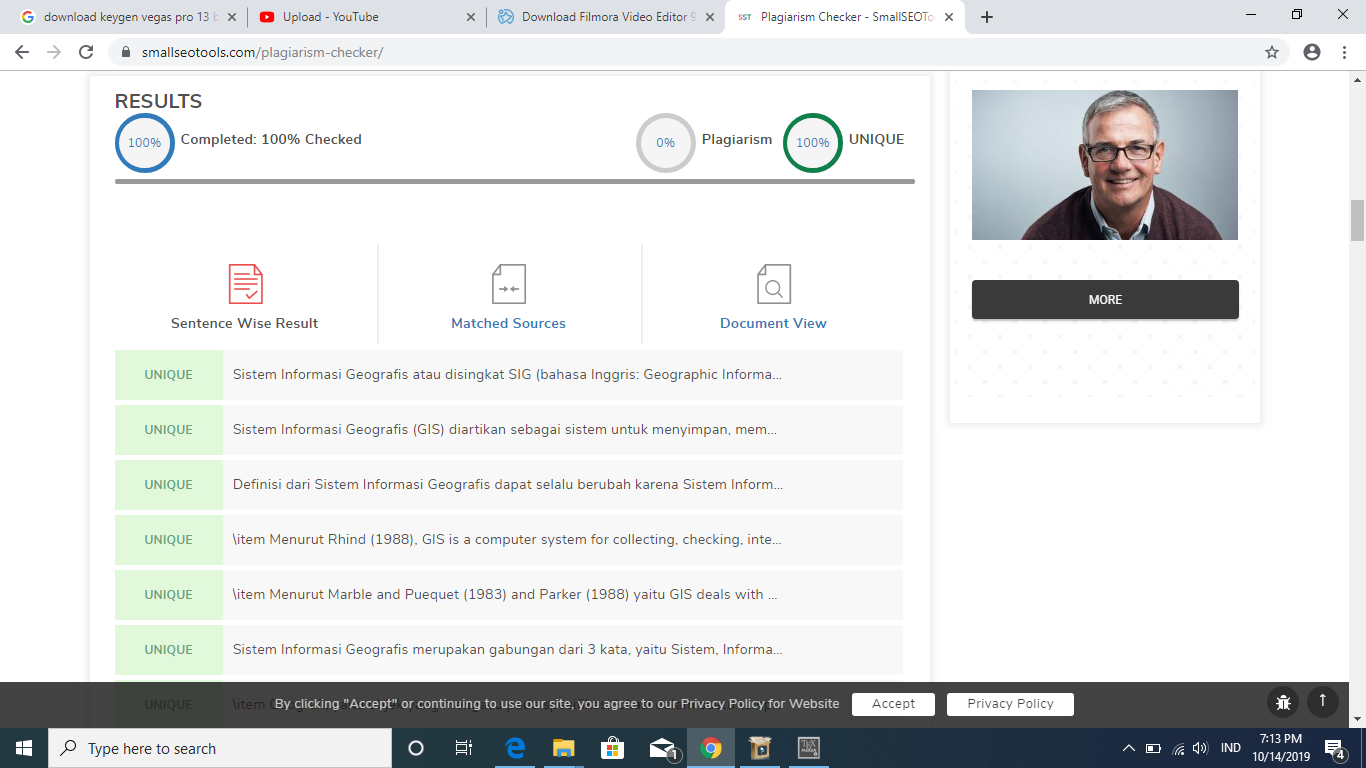
\includegraphics[width=4cm]{figures/Tugas1/1174054/plagiarismetgas1.png}
	\centering
	\caption{Gambar Plagiarisme}
\end{figure}